% ==============================================================================
% DOCUMENT HEADER
% ==============================================================================

\documentclass[11t, a4paper, twocolumn]{article} 
\usepackage[english]{babel}
\usepackage{microtype}
\usepackage{amsmath,amsfonts,amsthm}
\usepackage[svgnames]{xcolor}
\usepackage[hang, small, labelfont=bf, up, textfont=it]{caption}
\usepackage{booktabs}
\usepackage{lastpage}
\usepackage{graphicx}
\usepackage{enumitem}
\setlist{noitemsep}
\usepackage{sectsty}
\allsectionsfont{\usefont{OT1}{phv}{b}{n}}
\usepackage{lipsum}
\usepackage{geometry}
\geometry{
	top=1cm,
	bottom=1.5cm,
	left=2cm,
	right=2cm,
	includehead,
	includefoot
}
\setlength{\columnsep}{7mm}
\usepackage[T1]{fontenc}
\usepackage[utf8]{inputenc}
\usepackage{XCharter}
\usepackage{fancyhdr}
\pagestyle{fancy}
\renewcommand{\headrulewidth}{0.0pt}
\renewcommand{\footrulewidth}{0.25pt}
\renewcommand{\sectionmark}[1]{\markboth{#1}{}}
\lhead{}
\chead{\textit{\thetitle}}
\rhead{}
\lfoot{}
\cfoot{}
\rfoot{\footnotesize Page \thepage\ of \pageref{LastPage}}
\fancypagestyle{firstpage}{
	\fancyhf{}
	\renewcommand{\footrulewidth}{0pt}
}
\newcommand{\authorstyle}[1]{{\large\usefont{OT1}{phv}{b}{n}\color{Black}#1}}
\newcommand{\institution}[1]{{\footnotesize\usefont{OT1}{phv}{}{sl}\color{Black}#1}}
\usepackage{titling}
\newcommand{\HorRule}{\color{Black}\rule{\linewidth}{0.75pt}}
\pretitle{
	\vspace{-30pt}
	\HorRule\vspace{10pt}
	\fontsize{30}{34}\usefont{OT1}{phv}{b}{n}\selectfont
	\raggedright
	\color{Black}
}
\posttitle{\par\vskip 15pt}
\preauthor{}
\postauthor{
	\vspace{10pt}
	\par\HorRule
	\vspace{5pt}
}
\usepackage{lettrine}
\usepackage{fix-cm}
\newcommand{\initial}[1]{
	\lettrine[lines=3,findent=4pt,nindent=0pt]{
		\color{DarkGoldenrod}
		{#1}
	}{}
}
\usepackage{xstring}
\newcommand{\lettrineabstract}[1]{
	\StrLeft{#1}{1}[\firstletter]
	\initial{\firstletter}\textbf{\StrGobbleLeft{#1}{1}}
}
\usepackage[backend=bibtex,style=numeric,natbib=true]{biblatex}
\addbibresource{ref.bib}
\usepackage[autostyle=true]{csquotes}


\title{Estimating real-time high street footfall from Wi-Fi probe requests}
\author{
	\authorstyle{
		Balamurugan Soundararaj\textsuperscript{1}, 
		James Cheshire\textsuperscript{1} and 
		Paul Longley\textsuperscript{1}}
	\newline\newline
	\textsuperscript{1}\institution{
		Department of Geography, 
		University College London, 
		United Kingdom}
}
\date{\today}

% ==============================================================================
% DOCUMENT BODY
% ==============================================================================

\begin{document}

	\maketitle
	\thispagestyle{firstpage}

	In the past decade, Wi-Fi has emerged as the most commonly used technology in providing internet access to mobile devices such as smartphones, tablets and laptops in public and private spaces. This has resulted in multiple Wi-Fi networks being available at almost every location in urban environments. Traversing through this overlapping mesh of Wi-Fi networks, modern mobile devices with Wi-Fi antennae regularly broadcast a special type of signal known as probe requests, in order to discover available Wi-Fi networks and switch seamlessly between them. This is a hardware level signal which was standardised by IEEE 802.11b/g specification, to relay information about the source mobile device to any Access Point (AP) available around it. Since this is the first step in establishing a connection between any two devices, it is a standard feature of any device which uses a Wi-Fi radio to communicate. This makes these probe requests an open, passive, continuous, and wireless source of data available at any urban location. Moreover, the data can provide us with clues to understand the number of people present in the immediate surrounding in real-time and with high granularity \citep{freud2015,konto2017}. In this paper, using a set of probe requests collected at a high street location in London along with manually counted data, we demonstrate that pedestrian footfall can be estimated with considerable accuracy without infringing on the privacy of the mobile users involved.

	\begin{figure*}
		\begin{center}
			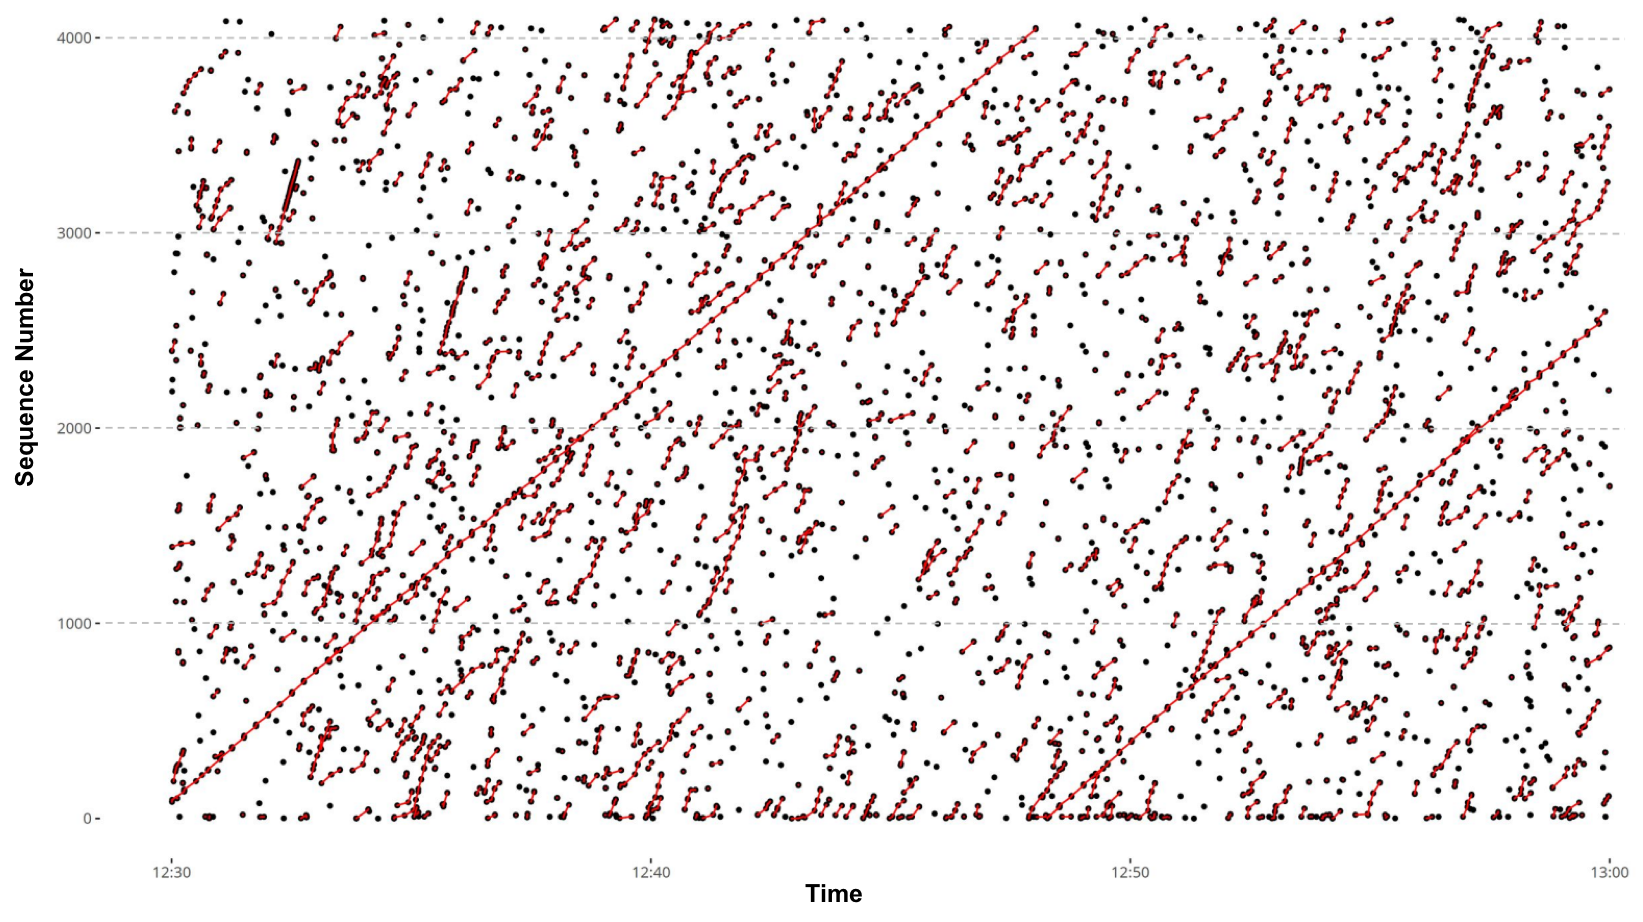
\includegraphics
				[width=0.8\textwidth,trim=4 4 4 4,clip]
				{outputs/clustering_2.png}
			\caption{Clustering probe requests based on increasing sequence
			numbers present in them.}
			\label{fig}
		\end{center}
	\end{figure*}

	There have been numerous attempts at using Wi-Fi to measure the volume and movement of people in the built environment for various applications \citep{zarim2006,sap2015,reki2007}. Though most research obtains feasible and favorable results, in recent years, one of the major challenges faced in such attempts has been the MAC address randomisation process. This process aims to protect the users’ privacy by anonymising the only globally identifiable portion of the probe requests, which results in a set of probe requests generated by the same device with different random MAC addresses \citep{green2008}. There have been various successful attempts by researchers to breaking this randomisation process in order to extract real MAC addresses, \citep{martin2017} but this usually results in serious risk of infringement of the privacy of the users of the mobile devices. There is a clear gap in the research for exploring methodologies which enable us to estimate the number of unique mobile devices from a set of anonymised probe requests, without the need to reveal their original MAC addresses.

	A pilot survey was conducted on Oxford Street in London in December 2017, where two sets of data were collected on pedestrian footfall. These datasets were collected through Wi-Fi sensing and manual counting in parallel. The Wi-Fi sensor collected all the probe requests which were broadcast around the area, and recorded the following data: the time-stamp at which they were collected, the MAC address of the source mobile device (anonymised using a hashing algorithm), the organisationally unique identifier (OUI) of the manufacturer of the device, the total length of the signal in bits, the strength of the signal reported by the mobile device in dBm, the sequence number of the signal, the duration for which the signal was transmitted, the service set identifier (SSID) of the access point targeted by the probe request, and the length of the extra information (tags) embedded in the packets. The manual count was undertaken using an Android application on a mobile phone: the researcher touched the phone’s screen every time an individual pedestrian footfall was counted, and this was recorded as a time-stamp. 

	Being located at one of the busiest retail locations in the United Kingdom, the WiFi sensor captured approximately 60,000 probe requests over a 30 minutes interval, and 3,722 people were counted manually. When we aggregated the probe requests by their MAC address for every minute, the difference between the sensor counts and the manual counts was observed to be on average 425\%. This suggested that there was a large amount of noise in the data which might have included signals from devices outside the area where themanual count was conducted, as well as anonymised probe requests from the same devices but with different MAC addresses. An initial analysis revealed that the fields - SSID and tags - were very sparse and did not provide much information for our cleaning process. In addition, the duration field was closely related to the length of the probe request and provides no new information. Therefore, we removed these fields from further analysis.

	We eliminated the noise from devices outside the area of interest by removing all the probe requests which reported a "low" signal strength. This classification of "high" vs "low" was performed using a k-means classification algorithm. The cut-off point for the collected data was -71 dBm. This process of filtering was highly effective and reduced the difference between the sensor counts and manual counts to 30\%. We observed that around 55\% of all probe requests collected were anonymised. We assigned the hashed MAC address the unique identifier for the remaining 45\% and investigated the anonymised probe requests further.

	We then used the fields - OUI, lengths and sequence number - to tackle the noise from devices which anonymised the probe requests. OUI and length were used to split the dataset into groups of probe requests from similar devices, and each subset was classified further using a graph based clustering algorithm where each cluster corresponded to a unique device. The algorithm created a graph where the probe requests represented the nodes, and links are created between them based on the following rules: 
		
	\begin{enumerate}
		\item A link could go only forward in time. 
		\item A link could exist between nodes with a maximum time difference of $\alpha$ (time threshold).
		\item A link could go from low to high sequence numbers.
		\item A link could exist between nodes with a maximum sequence number difference of $\beta$ (sequence threshold).
		\item A node could have only one incoming link and one outgoing link, which is the shortest of all such possible links.
	\end{enumerate}

	The nodes were then classified based on the unique connected component they belonged to. This classification was assigned as the unique identifier for the anonymised probe requests. Figure \ref{fig} shows the clustering process: the black dots show the probe requests and the red lines connect them into clusters representing those which were generated by the same device. We finally combined both normal and anonymised probe requests, aggregated them based on their unique identifier, and removed repeating probe requests which reduced the difference between the sensor counts and the manual counts to -18\%.

	It is important to note that the filtering process was done based soley on the information present in the probe requests and their temporal distribution. This ensured that although the mobile devices were uniquely identified, there was no further personal data generated by linking the probe requests to the users of the mobile devices. This method essentially gave us a way to estimate the footfall in real-time without identifying or tracking the mobile devices themselves.

	This Wi-Fi based footfall counting methodology offers a large number of applications and benefits for real time spatial analysis. Since Wi-Fi based sensors are inexpensive and the data model is scalable, it is possible to use this methodology for a large network of sensors to gather granular data on pedestrian footfall. Projects such as SmartStreetSensors \citep{sss2016}, may utilise this methodology to overcome the challenges introduced by the implementation of MAC address randomisation. Such precise and granular data also enables us to confidently model the pedestrian flow in urban road networks, and will be an indispensable tool in the smart city framework. It can also be used to understand and classify geographical areas based on the spatio-temporal distribution of the volume of activity in them.

	\printbibliography[title={References}]

\end{document}
